\chapter{Kế hoạch tổng thể (BPP)}
\label{Chapter2}

\section{Mô tả sản phẩm}
\subsection{Quy định sản phẩm}
\paragraph{Sản phẩm:} Hệ thống thông tin quản lý nhân sự - tiền lương dưới dạng 1 website, bao gồm các module như quản lý nhân sự, chấm công, tiền lương, báo cáo chi phí
\paragraph{Yêu cầu phi chức năng:}
\begin{itemize}
    \item Giao diện đẹp, đơn giản, dễ sử dụng: Giao diện người dùng cần phải rõ ràng, dễ hiểu và dễ dàng thao tác, không yêu cầu người dùng có kỹ năng công nghệ cao
    \item Đáp ứng nhu cầu của công ty: Hệ thống cần đảm bảo đáp ứng đầy đủ nhu cầu quản lý nhân sự và tiền lương của công ty, với các tính năng và chức năng phù hợp với các quy trình nội bộ của công ty
    \item Hiển thị chính xác, chi tiết: Thông tin trong hệ thống phải được hiển thị chính xác và chi tiết, bao gồm các thông tin về nhân sự, chấm công, tiền lương, và các báo cáo liên quan
    \item Dễ dàng nâng cấp và mở rộng: Hệ thống cần được thiết kế với khả năng mở rộng trong tương lai, để có thể tích hợp các tính năng mới hoặc nâng cấp khi cần thiết mà không gây gián đoạn quá trình vận hành hiện tại
\end{itemize}
\paragraph{Yêu cầu chức năng:}
\begin{itemize}
    \item Chức năng người quản lý:
    \begin{itemize}
        \item \textbf{Đăng nhập và đăng xuất:} Người quản lý cần có quyền truy cập vào hệ thống bằng tài khoản cá nhân và có thể đăng xuất sau khi hoàn thành công việc
        \item \textbf{Quản lý nhân sự:} Hệ thống phải cho phép người quản lý thêm, sửa, xóa thông tin nhân viên, cũng như theo dõi thông tin cá nhân, chức vụ, phòng ban, v.v
        \item \textbf{Quản lý chấm công:} Người quản lý có thể theo dõi và chỉnh sửa thời gian làm việc của nhân viên, xử lý các vấn đề liên quan đến việc điểm danh, vắng mặt, và các chế độ nghỉ phép
        \item \textbf{Quản lý tiền lương:} Hệ thống cho phép người quản lý tính toán và phê duyệt tiền lương của nhân viên dựa trên các yếu tố như số giờ làm việc, mức lương cơ bản, thưởng, khấu trừ, v.v
        \item \textbf{Quản lý lịch làm việc:} Cung cấp chức năng để quản lý lịch làm việc của nhân viên, lập lịch cho các ca làm việc, nghỉ phép, v.v
        \item \textbf{Thống kê và báo cáo:} Người quản lý có thể truy xuất các báo cáo tài chính liên quan đến chi phí nhân sự, lương thưởng, và các báo cáo thống kê khác để phục vụ cho việc quản lý và ra quyết định
    \end{itemize}
\end{itemize}
\subsection{Đặc trưng sản phẩm}
\begin{itemize}
\item \textbf{Tự động hoá quản lý nhân sự và tiền lương:} Hệ thống sẽ giúp giảm thiểu công việc thủ công trong việc tính toán và quản lý lương thưởng của nhân viên, từ đó tăng cường độ chính xác và giảm thiểu sai sót
\item \textbf{Quản lý nhân sự hiệu quả:} Cho phép người quản lý theo dõi các thông tin về nhân viên như lịch sử công tác, thông tin cá nhân, phòng ban, chức vụ, v.v. Từ đó giúp cải thiện quá trình ra quyết định và tối ưu hóa các quy trình nhân sự
\item \textbf{Quản lý tiền lương chính xác:} Tính toán lương, thưởng, các khoản khấu trừ, và các yếu tố khác liên quan đến tiền lương của nhân viên một cách tự động và chính xác, giúp giảm thiểu sai sót trong các báo cáo tài chính
\item \textbf{Thống kê tài chính dễ dàng hơn:} Cung cấp các công cụ phân tích và báo cáo để người quản lý dễ dàng theo dõi chi phí nhân sự và lập các báo cáo tài chính liên quan, phục vụ cho các mục đích quản lý và báo cáo thuế
\item \textbf{Tăng hiệu quả công việc:} Hệ thống sẽ giúp người dùng tiết kiệm thời gian và công sức trong công tác quản lý nhân sự và tiền lương, từ đó tạo điều kiện để tập trung vào các hoạt động quan trọng khác trong công ty
\end{itemize}
\subsection{Đặc trưng sản phẩm}
\begin{itemize}
    \item Nhân viên quản lý 
    \item Máy chấm công
    \item Thư điện tử
    \item Hệ thống thanh toán 
    \item Hệ thống kế toán
    \item Nhân sự
\end{itemize}
\subsection{Đặc trưng sản phẩm}
\begin{figure}[H]
    \centering
    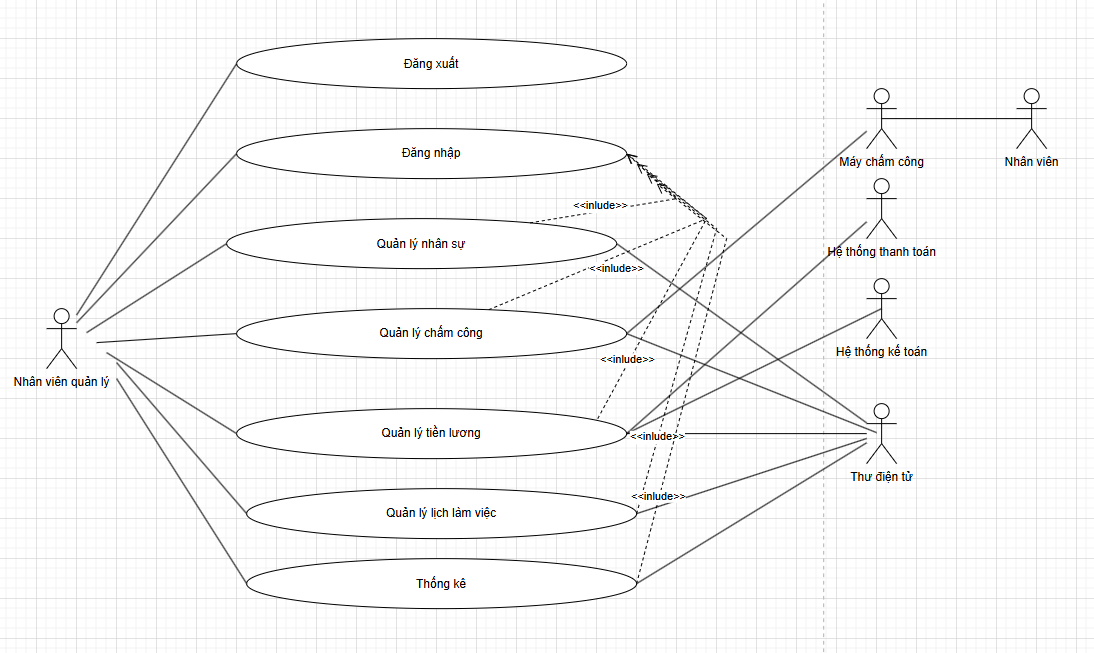
\includegraphics[width=\textwidth]{images/usecase.png}
    \caption{Usecase tổng quát của hệ thống}
    \label{fig:usecase-tong-quat}
\end{figure}

\section{Mô hình xây dựng}
\subsection{Phương án 1: chọn mô hình Scrum}
\paragraph{Giới thiệu mô hình:}
\begin{itemize}
    \item Scrum là phương pháp phát triển phần mềm linh hoạt theo mô hình Agile, giúp đội dự án có thể thích ứng nhanh với thay đổi từ khách hàng và kiểm soát tiến độ hiệu quả. Scrum được thiết kế để xử lý các dự án có yêu cầu phức tạp, với ít thông tin ban đầu hoặc yêu cầu có thể thay đổi
\end{itemize}
\paragraph{Ưu điểm:}
\begin{itemize}
    \item Dễ dàng thích ứng với thay đổi trong yêu cầu
    \item Có sự cộng tác chặt chẽ giữa các bên
    \item Sản phẩm được phát triển và kiểm thử liên tục, giảm thiểu rủi ro
\end{itemize}
\paragraph{Nhược điểm:}
\begin{itemize}
    \item Yêu cầu khách hàng tham gia xuyên suốt dự án
    \item Phù hợp với các dự án có yêu cầu linh hoạt, không thích hợp với yêu cầu cố định
\end{itemize}
\subsection{Phương án 2: mô hình thác nước (Waterfall)}
\paragraph{Giới thiệu mô hình:}
\begin{itemize}
    \item Mô hình Thác Nước là quy trình phát triển phần mềm tuyến tính, các giai đoạn được thực hiện tuần tự và không thay đổi khi đã chuyển sang bước tiếp theo
\end{itemize}
\paragraph{Ưu điểm:}
\begin{itemize}
    \item Quy trình rõ ràng, có thể đo lường tiến độ dự án dễ dàng
    \item Phù hợp với các dự án có yêu cầu cụ thể và cố định từ đầu
    \item Tiết kiệm thời gian và chi phí cho các dự án quy mô nhỏ, ít thay đổi
\end{itemize}
\paragraph{Nhược điểm:}
\begin{itemize}
    \item Khó thích ứng với yêu cầu thay đổi của khách hàng trong quá trình phát triển
    \item Lỗi phát hiện ở giai đoạn cuối sẽ tốn kém chi phí và thời gian sửa chữa
    \item Khách hàng chỉ thấy sản phẩm hoàn chỉnh khi kết thúc dự án
\end{itemize}
\subsection{Kết luận về phương án lựa chọn}
\begin{itemize}
    \item Do yêu cầu dự án đã cố định và rõ ràng, quy mô nhỏ: Áp dụng mô hình Thác Nước
    \begin{figure}[H]
        \centering
        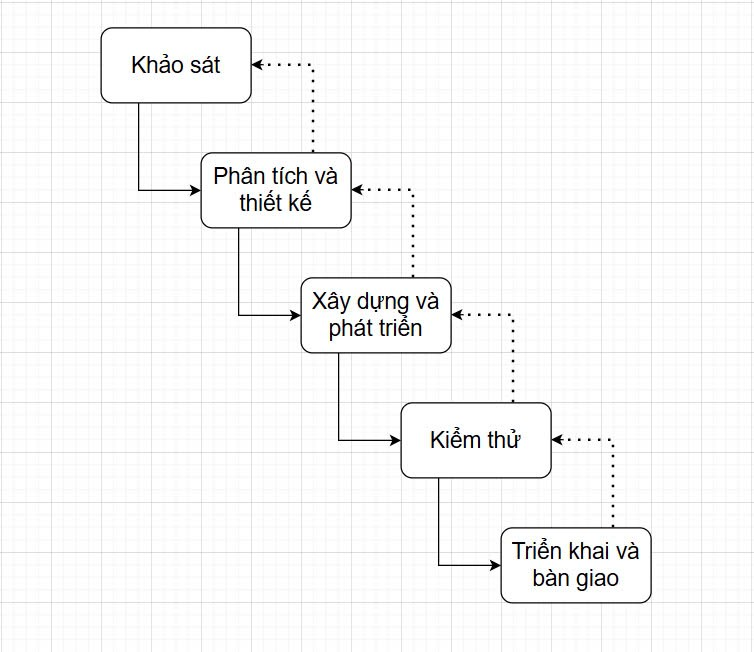
\includegraphics[width=\textwidth]{images/waterfall.png}
        \caption{Mô hình thác nước}
        \label{fig:usecase-tong-quat}
    \end{figure}
\end{itemize}

\section{Phạm vi công việc dự án}
\begin{itemize}
    \item Phạm vi:
\begin{itemize}
    \item Khảo sát
    \item Phân tích và thiết kế
    \item Xây dựng và phát triển hệ thống
    \item Xây dựng và phát triển hệ thống sau kiểm thử
    \item Xây dựng và phát triển hệ thống sau triển khai và chuyển giao
\end{itemize}
\end{itemize}
\begin{itemize}
\item Ngoài phạm vi:
\begin{itemize}
    \item Bảo trì, Nâng cấp
    \item Phát triển hệ thống ở các dạng khác như mobile app, desktop app
\end{itemize}
\end{itemize}

\section{Lịch trình dự án}
\subsection{Khảo sát}
\begin{itemize}
    \item \textbf{Thời gian(5 ngày):} 24/11/2024 - 28/11/2024
    \item \textbf{Công việc:}
    \begin{itemize}
        \item Khảo sát yêu cầu chức năng và phi chức năng (3 ngày): 24/11/2024 - 26/11/2024
        \item Khảo sát quy trình nghiệp vụ (1 ngày): 27/11/2024
        \item Tổng hợp, lập hồ sơ khảo sát (1 ngày): 28/11/2024
    \end{itemize}
    \item \textbf{Thành viên được phân công:} Quang, Phong, Phương, Phát
    \item \textbf{Sản phẩm:} Hồ sơ khảo sát
    \item \textbf{Ước lượng chi phí:} 4.400.000 VND
\end{itemize}
\subsection{Phân tích và thiết kế}
\begin{itemize}
    \item \textbf{Thời gian(13 ngày):}  29/11/2024 - 11/12/2024
    \item \textbf{Công việc:}
    \begin{itemize}
        \item Phân tích quy trình nghiệp vụ (2 ngày): 29/11/2024-30/11/2024
        \item Phân tích yêu cầu (2 ngày): 01/12/2024 - 02/12/2024
        \item TThiết kế kiến trúc hệ thống (2 ngày): 03/12/2024-04/12/2024
        \item Thiết kế CSDL (3 ngày): 05/12/2024 - 07/12/2024
        \item Thiết kế giao diện (4 ngày): 08/12/2024 - 11/12/2024
        \item Lập hồ sơ phân tích thiết kế (1 ngày): 11/12/2024
    \end{itemize}
    \item \textbf{Thành viên được phân công:} Tất cả thành viên
    \item \textbf{Sản phẩm:} Hồ sơ phân tích thiết kế
    \item \textbf{Ước lượng chi phí:} 19.400.000 VND
\end{itemize}
\subsection{Xây dựng và phát triển hệ thống}  
\begin{itemize}
    \item \textbf{Thời gian(17 ngày):} 12/12/2024 - 28/12/2024
    \item \textbf{Công việc:}
    \begin{itemize}
        \item Xây dựng và phát triển CSDL (4 ngày): 12/12/2024 - 15/12/2024
        \item Xây dựng và phát triển Front-end (6 ngày): 16/12/2024 - 21/12/2024
        \item Xây dựng và phát triển Back-end (7 ngày): 22/12/2024 - 28/12/2024
        \item Tích hợp mã nguồn đa tầng (1 ngày): 28/12/2024
    \end{itemize}
    \item \textbf{Thành viên được phân công:} Tất cả thành viên
    \item \textbf{Sản phẩm:} Phần mềm sau tích hợp 
    \item \textbf{Ước lượng chi phí:} 32.400.000 VND
\end{itemize}
\subsection{Xây dựng và phát triển hệ thống sau kiểm thử}
\begin{itemize}
    \item \textbf{Thời gian(8 ngày):} 29/12/2024 - 05/01/2024
    \item \textbf{Công việc:}
    \begin{itemize}
        \item Kiểm thử và sửa lỗi (8 ngày): 29/12/2024 - 05/01/2025 
        \item Lập hồ sơ kiểm thử (1 ngày): 5/01/2025
    \end{itemize}
    \item \textbf{Thành viên được phân công:} Quang,Phát
    \item \textbf{Sản phẩm:} Hồ sơ kiểm thử, Phần mềm sau kiểm thử
    \item \textbf{Ước lượng chi phí:} 4.800.000 VND
\end{itemize}
\subsection{Xây dựng và phát triển hệ thống sau triển khai và chuyển giao}
\begin{itemize}
    \item \textbf{Thời gian(5 ngày):} 06/01/2025 - 10/01/2025
    \item \textbf{Công việc:}
    \begin{itemize}
        \item Viết tài liệu hướng dẫn (1 ngày): 06/01/2025
        \item Chuyển giao cài đặt và Đào tạo sử dụng (2 ngày): 7/1/202025-08/1/2025
        \item Lập hồ sơ triển khai và chuyển giao (2 ngày):  09/01/2025-10/01/2025
    \end{itemize}
    \item \textbf{Thành viên được phân công:} Phương, Hải, Quang
    \item \textbf{Sản phẩm:} Hồ sơ triển khai và bàn giao, Hệ thống sau khi triển khai và chuyển giao
    \item \textbf{Ước lượng chi phí:} 4.600.000 VND
\end{itemize}

\section{Chi phí dự án}
\begin{itemize}
    \item \textbf{Chi phí dự kiến:} 260.000.000 VND
    \item \textbf{Đầu mục chi phí:}
    \begin{itemize}
        \item Tài sản cố định: 15.000.000 VND
        \item Chi phí vận hành: 153.000.000 VND
        \item Chi phí phần mềm: 30.000.000 VND
        \item Phúc lợi và các hoạt động khác: 62.000.000 VND
    \end{itemize}
\end{itemize}